\section{Graphical representation}

$3$-valued structures are displayed using graphical
representation. For example an input structure for the reverse
function is given in \figref{ManReverseTVS}.

\begin{figure}
\begin{center}
\begin{minipage}[t]{.33\linewidth}
%\vspace*{4cm}
\begin{tabbing}
\%n = \{head, tail\}\\
\%p =\=\+\ \{\\
      sm = \{tail:1/2\}\\
      n = \{head\deref tail:1/2, tail\deref tail:1/2\}\\
      x = \{head\}\\
      t[n] = \{head\deref head, head\deref tail, tail\deref tail:1/2\}\\
      r[n,x] = \{head, tail\}\-\\
\}
\end{tabbing}
\end{minipage}\hfill
\begin{minipage}[t]{.33\linewidth}
\vspace*{0mm} 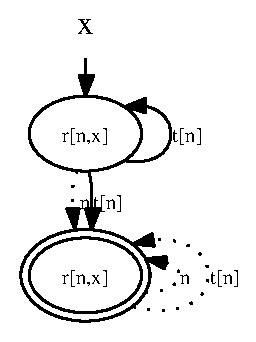
\epsfig{file=sll_tvs,width=3cm}
\end{minipage}
\end{center}
\caption{\label{Fi:ManReverseTVS}The TVS of an input structure for
the reverse function analysis and its graphical representation.}
\end{figure}

\subsection{Colors}

Colors are used to represent the different values for predicates.
Solid black is true ($1$), dotted black is unknown ($1/2$), and
red is false ($0$).

\subsection{Shapes}

The values of nullary predicates are displayed in a box titled
``nullary''.  By default, nullary predicates with true values are
written inside the box, nullary predicates with false values, are
not shown and nullary predicates with indefinite values ($1/2$)
have the value added next to them.

An ellipse represents a node.  If the ellipse is double-circled
then the node is a summary node, and if it is green then the node
is maybe active ($ac=1/2$).  Unary predicates are written within
the ellipse.  If the value is different from $1$ it is appended to
predicate's name (i.e., $=0$ or $=1/2$).


\subsection{Edges}

Binary predicates are represented as directed arrows between the
left and right arguments and annotated by the name of the
predicate.  If a binary predicate has the same value for both
$u_1\deref u_2$ and $u_2\deref u_1$ the two edges are replaced
with a bidirectional edge.
